\chapter{Einführung}\label{ch:intro}

Das Smartphone ist heutzugtage der stete Begleiter eines Menschen. \enquote{Zwei Drittel der Bevölkerung und nahezu jeder 14- bis 29-Jährige geht darüber ins Netz.} \cite{usage} Auch die Prognose zeigt, das der Absatzmarkt immer weiter steigen wird (Abbildung \ref{fig:prognose_fig}).

\begin{figure}[H]
	\begin{center}
		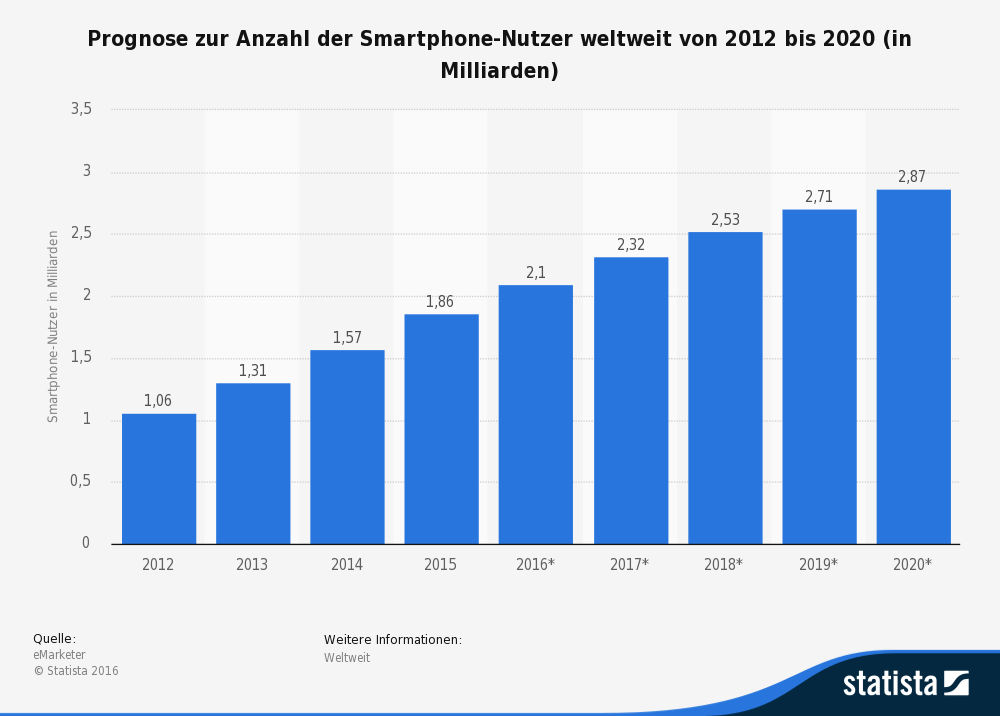
\includegraphics[width=0.86\textwidth]{images/prognose-zur-anzahl-der-smartphone-nutzer-weltweit-bis-2020.png}
		\caption{Prognose zur Anzahl der Smartphone-Nutzer weltweit von 2012 bis 2020 (in Milliarden) \cite{prognose}}
		\label{fig:prognose_fig}
	\end{center}
\end{figure}

Umso wichtiger ist es das die Softwareentwicklung diesen Trend ernst nimmt. Der ehemalige Google-Chef Eric Schmidt sagte bereits 2010: \enquote{Googles Devise heißt jetzt \enquote{Mobile first}}. 
Diese Devise wird auch heute noch von vielen Unternehmen verfolgt, das ist der Grund weswegen in den einzelnen Stores heutzutage so viele Apps angeboten werden. Bei Android im Playstore sind es im Oktober 2016 ca 2.432.000 Apps \cite{play_store}, bei Apple im App Store sind es ca 2.000.000 Apps (Stand Juni 2016) \cite{app_store}. Neben Googles Android und Apples IOs gibt es noch andere Betriebssysteme, wie Microsofts Windows Phone oder Blackberrys Blackberrys OS und noch ein paar andere. Jedoch bestimmen die beiden erstgenannten Systeme den Markt (Abbildung \ref{fig:os_fig}).

\begin{figure}[H]
	\begin{center}
		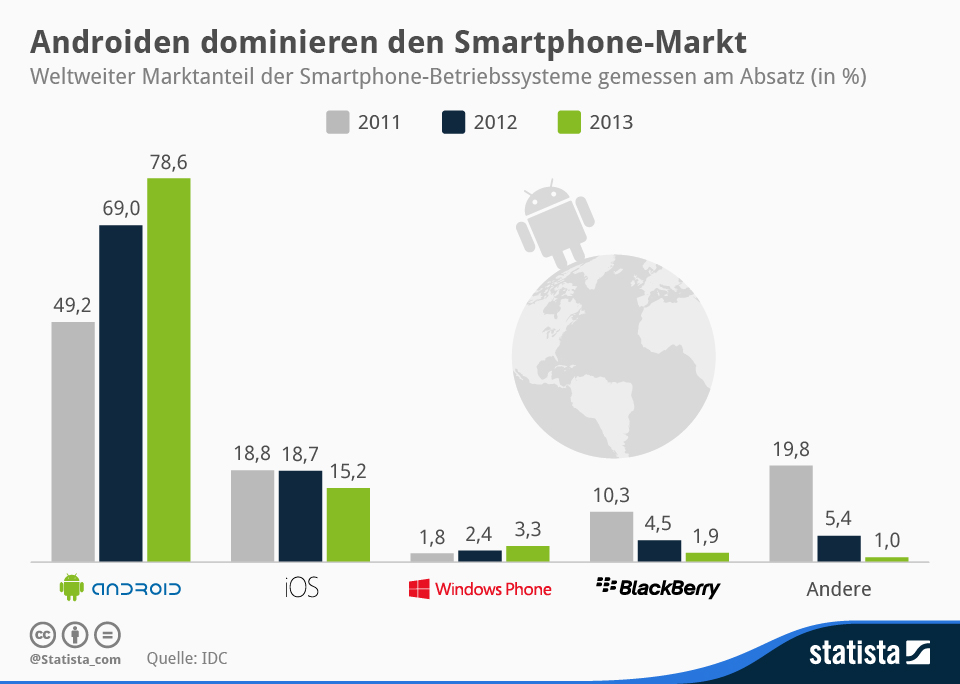
\includegraphics[width=0.86\textwidth]{images/os.jpg}
		\caption{Der weltweite Marktanteil von Smartphone-Betriebssysteme. \cite{os}}
		\label{fig:os_fig}
	\end{center}
\end{figure}

Ein großes Problem in dieser Branche ist die ernorme Schnelllebigkeit. Vor allem im Bereich Android werden beinahe wöchentlich neue Geräte durch unterschiedliche Hersteller vorgestellt. Neben den hardware-spezifischen Unterschieden wie: Größe und Auflösung des Displays, Größe des verbauten RAMs, Prozessorleistung und so weiter, muss ein Entwickler für Android Applikations zusätzlich noch mit den hersteller-spezifischen Eigenentwicklungen von Android kämpfen. So nutzt zum Beispiel HTC, ihre HTC Sense \cite{htc_sense}, Samsung setzt auf TouchWiz \cite{touchwiz}. Neben diesen herstellergebundenen Systeme gibt es zusätzlich noch Custom-ROMs, welche durch den Nutzer selbst installiert werden können. Die beliebtesten ROMs sind Paranoid Android und CyanogenMod \cite{rom}. Jedes dieser Systeme besitzt auserdem noch unterschiedliche Versionen so befindet sich Vanilla Android im Moment in der Version 7.0 Nougat.
Durch die einzelnen Systeme und deren Versionen entstehen ernorm viele Anforderungen an die Software, welche möglichst eine Vielzahl der Varianten unterstützen sollte. Um diese Anforderungen stemmen zu können, muss ein extrem hoher Anteil an Wartung in die Entwicklung und Instandhaltung einfließen. Zusätzlich zu dem Mehraufwand muss sich der Android-Entwickler ständig über die neuen Spezifikationen informieren.

\section{Motivation}\label{sec:motivation}
Aus der Analyse der \enquote{Top 20 Android-Smartphone-Apps in Deutschland} \cite{top_apps} geht hervor das bei den meisten Applikationen mehr oder weniger die gleichen Grundfunktionen verwendet werden:
\begin{itemize}
	\item Anzeigen von nachgeladenen Daten.
	\item Neue Daten zum Backend senden.
	\item Bestehende Daten manipulieren.
	\item Bestehende Daten löschen.
\end{itemize}

Jedoch sind diese Implementierungen der Grundfunktionen so in die einzelnen Applikationen verwoben, das sie jedes mal neu Implementiert werden müssen. Es geht sogar noch weiter, nehmen wir zum Beispiel eine Kampus-App, hier werden ganze Designkomponenten mehrfach implementiert. Die meisten dieser Kampus-Apps besitzt eine View, welche eine Liste aller Dozenten anzeigt, oder es gibt die Möglichkeit einen Dozenten im Detail zu betrachten. Dafür muss jedesmal eine Businesslogik geschrieben werden, die sich kaum von einer anderen Applikation unterscheidet. Auch muss sich der Entwickler jedes mal um das Design gedanken machnen. 

Diese Arbeit soll nun Lösungsansätze erarbeiten, welche den oben genannten Mehraufwand reduzieren kann. Der Entwickler von neuen Applikationen oder von Erweiterungen soll sich auf spezifische Anforderungen konzentrieren können und den allgemeinen Teil generieren lassen.
Auch die Wartung der allgemeinen Teile wird durch die Generierung vereinfacht. Da diese nur einmalig vorgenommen werden muss und dann in allen anderen Applikationen übernommen werden kann.

\section{Zielsetzung}\label{sec:target}
Das Ziel dieser Ausarbeitung liegt darin, das der Leser ein grundsätzliches Verständnis in der Implementierung von Custom Views in Android, Erstellung von AAR-Bibliotheken und der Datenkommunikation mittels einer REST-API erlangen. Mit diesem Wissen, sollte der Leser dann in der Lage sein Generatoren für Custom Views zu entwickeln, welche die oben genannten Grundfunktionen einer Applikation abdecken.\\
Darüber hinaus soll auch ein Gefühl dafür entwickelt werden, wann es Sinn macht eine View als Custom View zu implementieren und wann der benötigte Mehraufwand nicht mehr in Relation zu einem vernünftigen Ergebniss steht.


\section{Aufbau der Arbeit}\label{sec:structure}
Aufbau